\documentclass[tikz,crop]{standalone}

\usepackage{tikz}
\usepackage{xcolor}
\usepackage{pgfplots}
%\usepackage{tikz-uml}

\pgfplotsset{compat=1.18}
\usepgfplotslibrary{statistics}

\usetikzlibrary{shapes,arrows,positioning,backgrounds,calc,intersections,calc,svg.path,fit}

\definecolor{ugent-re}{RGB}{220, 78, 40}        % vermilion			/ vermiljoen
\definecolor{ugent-we}{RGB}{45, 140, 168}       % no match
\definecolor{ugent-ge}{RGB}{232, 94, 113}       % rose				/ bleekrood
\definecolor{ugent-ea}{RGB}{111, 113, 185}      % distant blue		/ verblauw
\definecolor{ugent-pp}{RGB}{251, 126, 58}       % deep orange		/ dieporanje
\definecolor{ugent-ps}{RGB}{113, 168, 96}       % yellow green		/ geelgroen

\tikzstyle{python}=[fill=ugent-ps!50!white]
\tikzstyle{java}=[fill=ugent-we!50!white]
\tikzstyle{haskell}=[fill=ugent-ea!50!white]
\tikzstyle{js}=[fill=ugent-pp!50!white]
\tikzstyle{c}=[fill=ugent-re!50!white]

\newlength{\block}
\setlength{\block}{0.75cm}

\tikzstyle{a}=[anchor=north west]
\tikzstyle{box}=[a,draw,rectangle]
\tikzstyle{node}=[a,draw,minimum height=0.5cm,align=center,fill=white,text depth=.25ex]
\tikzstyle{document}=[node,tape,tape bend top=none]
\tikzstyle{cont}=[box,minimum height=1\block,minimum width=1\block]
\tikzstyle{arrow}=[draw, -latex]
\tikzstyle{inner}=[box,draw=gray]

% Blue box style
\tikzstyle{bluebox}=[draw=ugent-we,java]
\tikzstyle{redbox}=[draw=ugent-re,c]
\tikzstyle{greenbox}=[draw=ugent-ps,python]

% Some things specific to TESTed imagery.
\tikzstyle{tc}=[box,draw=ugent-ps]
\tikzstyle{comp}=[box,draw=ugent-re,fill=ugent-re,fill opacity=0.05]
\tikzstyle{exec}=[box,draw=ugent-we,fill=ugent-we,fill opacity=0.10]

% Stuff from tested-engine/concept.tex
\tikzstyle{process}=[node,rectangle]
\tikzstyle{terminator}=[node,rectangle,rounded corners=0.5cm]
\tikzstyle{io}=[node,trapezium,trapezium left angle=70,trapezium right angle=-70,minimum width=2.5cm,trapezium stretches=true]
\tikzstyle{small}=[font=\footnotesize,color=darkgray]
\tikzstyle{submission}=[document,align=right,minimum width=3cm,minimum height=1cm,text depth=0.5cm,inner sep=0.5mm,font=\scriptsize]
\usepackage{siunitx}
\usepackage{scratch3}

% Stuff from chatper3/flow.tex
\tikzstyle{height}=[minimum height=0.75\block]
\tikzstyle{contt}=[cont,minimum height=0.75\block]
\tikzstyle{compop}=[comp,text opacity=1]
\tikzstyle{execop}=[exec,text opacity=1]

\tikzstyle{hnode}=[draw,anchor=center,minimum height=\block,text depth=.25ex,align=center]
\tikzstyle{executable}=[hnode,ultra thick,fill=gray!10]
\tikzstyle{inner-exec}=[node,anchor=center,minimum width=3.25\block,densely dotted,font=\footnotesize,fill=none]
\tikzstyle{stmt}=[node,anchor=center,fill=gray!30,minimum width=4.5\block,font=\footnotesize]
\tikzstyle{fieldset}=[minimum height=\block,fill=white,text depth=.5ex,fill=white]

\begin{document}

% Explicitly not [x=0.75cm,y=0.75cm] like the rest.
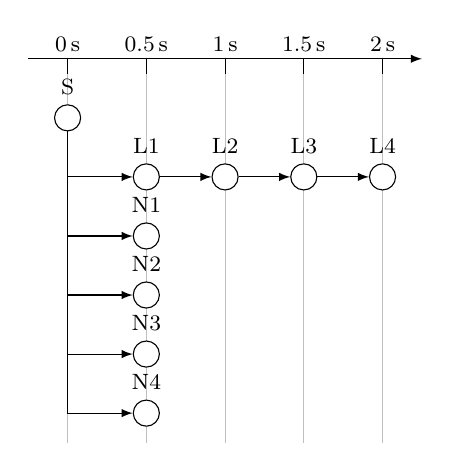
\begin{tikzpicture}[y=0.75cm]
  \draw [arrow] (-0.5,0) -- (4.5,0);

  \foreach \x in {0,...,4} {
    \draw[color=lightgray] (\x,0) -- (\x,-6.5);
    \draw (\x,0) -- (\x,-0.25);
  }

  \foreach \t [count=\x from 0] in {0,0.5,1,1.5,2} {
    \node at (\x,0.25) {\footnotesize\qty{\t}{\second}};
  }

  % Start event
  \node [draw,fill=white,circle,label={\footnotesize S}] (s) at (0,-1) {};

  % Linear
  \node [draw,fill=white,circle,label={\footnotesize L1}] (l1) at (1,-2) {};
  \node [draw,fill=white,circle,label={\footnotesize L2}] (l2) at (2,-2) {};
  \node [draw,fill=white,circle,label={\footnotesize L3}] (l3) at (3,-2) {};
  \node [draw,fill=white,circle,label={\footnotesize L4}] (l4) at (4,-2) {};

  \draw[arrow] (l1) -- (l2);
  \draw[arrow] (l2) -- (l3);
  \draw[arrow] (l3) -- (l4);

  % Non-linear
  \node [draw,fill=white,circle,label={\footnotesize N1}] (nl1) at (1,-3) {};
  \node [draw,fill=white,circle,label={\footnotesize N2}] (nl2) at (1,-4) {};
  \node [draw,fill=white,circle,label={\footnotesize N3}] (nl3) at (1,-5) {};
  \node [draw,fill=white,circle,label={\footnotesize N4}] (nl4) at (1,-6) {};

  \draw[arrow] (s) -- (s|-nl4) -- (nl4);
  \draw[arrow] (s|-nl3) -- (nl3);
  \draw[arrow] (s|-nl2) -- (nl2);
  \draw[arrow] (s|-nl1) -- (nl1);
  \draw[arrow] (s|-l1) -- (l1);
\end{tikzpicture}

\end{document}
